\documentclass[12pt]{article}

\usepackage{sbc-template}

\usepackage{graphicx,url}
\usepackage{rotating}
\usepackage{dcolumn}
\usepackage{float}
%\usepackage[brazil]{babel}   
\usepackage[latin1]{inputenc}  



%RENAMES
\renewcommand{\figurename}{Figura}
\renewcommand{\tablename}{Tabela}
\renewcommand{\refname}{Referências}
     
\sloppy

\title{Problema 4: "NOME DO PROBLEMA AQUI E EM UMA FIGURA AI"}

\author{Turma P04}


\address{MI - Projetos de Circuitos Digitais, Período 2015.1\\ Tutor: Marcos Paz\\
Curso de Engenharia de Computação \\ Universidade Estadual de Feira de Santana (UEFS)
}

\begin{document} 

\maketitle

\begin{resumo} 
O presente relatório descreve o processo de resolução do quarto problema do MI - Circuitos Digitais, da supracitada turma,no período de 2015.1, na Universidade Estadual de Feira de Santana. O problema propôs, dado o sucesso dos projetos pretéritos, que os estudantes desenvolvessem um protótipo do jogo Batalha Naval em \textit{FPGA}, tomando como base o  protótipo do controlador para matriz de \textit{LED}, sendo que a comunicação com este novo circuito deveria acontecer através de um computador pessoal utilizando o conceito de comunicação serial, tornando o projeto a ser desenvolvido, mais confiável em relação a transmissão de dados.
\end{resumo}

\section{Introdução} \label{sec:firstpage}

Hoje em dia cresce, substancialmente, a ampla utilização de jogos no segmento lúdico de simulação 2D. Estes são utilizados em diversas áreas conhecidas, tendo uma mais elevada utilização na educação. Além do papel que os mesmos podem fornecer à educação, podem servir , também, única e exclusivamente como forma de entretenimento entre os mais jovens, bem como para o público mais adulto. Um exemplo destes jogos, é famigerado Batalha Naval. Sendo no Brasil no ano de 1988, o jogo batalha naval é um dos jogos de maiores sucessos entre o público mundial. Em sua forma mais rústica, dois adversários desenhavam em folhas de papel, navios posicionados em um mar imaginário quadriculado, formando uma grade. Todavia, no contexto atual, além de encontrar versões deste jogo de maneira similar aos seus primórdios, encontra-se, também, aplicativos para diversas arquiteturas que executam o mesmo processo, facilitando assim a sua disseminação entre as pessoas.

Além da existência, como visto, deste tipo de jogo na forma de aplicativos móveis, existe a possibilidade, também, de desenvolvê-lo utilizando circuitos digitais, visando a criação de um jogo lúdico de simulação 2D.  É de se notar, que para desenvolvê-lo, faz-se necessário utilizar um conceito muito importante na eletrônica digital, a saber, memória RAM. A criação deste tipo de jogo, traz diversas vantagens para o empreendedor que o desenvolve, justamente pelo fato do mercado de jogos está sempre em constante expansão. lembrando que hoje em dia, aplicações envolvendo a tecnologia digital tem ampla aceitação no mercado, o ser humano necessita de recursos tecnológicos, com forma também de pertença, e inclusão no mundo global tecnológico. 

Desta forma, observando a mudança atual do mercado, principalmente no que diz respeito a alta receptividade em relação a jogos eletrônicos, o grupo Inova Digital Bahia S.A  resolveu adaptar o projeto desenvolvido anteriormente, para que o mesmo funcionasse como uma espécie de jogo Batalha Naval, seguindo um modelo de simulação $2D$. Sendo que este novo protótipo deveria ser controlado remotamente, a partir de um computador pessoal, enviando os dados por meio de canal de comunicação serial. Neste jogo, dois modos estarão disponíveis, o modo de gravação e o modo de jogo propriamente dito, cada modo contendo suas especificações e características próprias, as quais serão descritas nas seções posteriores.

É importante lembrar, que para desenvolver este projeto, foram utilizados além dos recursos já conhecidos, fez-se uso também de Máquinas de estados, registrador de descolocamento, porta serial, protocolo de comunicação RS-232, conversores de níveis elétricos e, por último, mas não menos importante, Software para comunicação com Hardware.

\section{Fundamentação Teórica}

Na seção que segue, serão descritos os conceitos utilizados para resolução do problema proposto, frisando os conceitos que foram de fundamental importância para solucionar o mesmo, tendo contribuição de maneira direta ou indireta.

\subsection{Máquinas de Estados}
Em se tratando de Circuitos Digitais, diversos dispositivos têm uma ampla importância, dentre estes dispositivos temos os conhecidos contadores, os quais segundo\cite{tocci1997digital} são Máquinas de estados específicas. Floyd, por sua vez, vai mais adiante, e fala que Máquinas de estados ou circuito sequencial é um circuito que  consiste de uma seção de lógica combinacional e uma seção de memória (flip-flops)\cite{floyd2011digital}. Na figura~\ref{fig:diagrama} podemos observar o circuito típico para uma máquina de estados. Vale acrescentar que a quantidade de estados que uma máquina pode interpretar é diretamente ligada a quantidade de Flip-Flop, a quantidade de estados pode ser obtido fazendo $2^{n}$, sendo n o número de Flip-flops.  

\begin{figure}[!htbp]
\centering
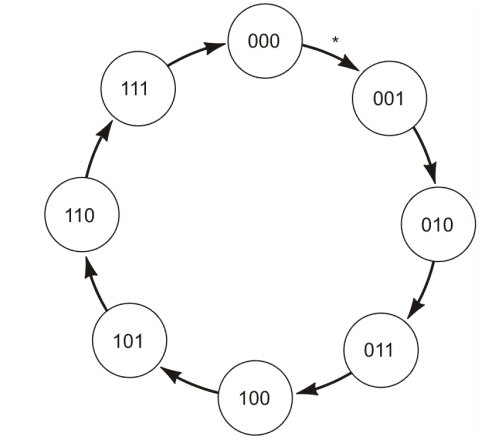
\includegraphics[width=.5\textwidth]{img/p4/diagrama-estados.png}
\caption{Diagrama de estados de um contador de 3 bits\cite{floyd2011digital}}
\label{fig:diagrama}
\end{figure}

Existem basicamente, dois modelos de máquinas de estados, a saber, máquina Moore e máquina Mealy. Na máquina Moore, a saída depende única e exclusivamente dos seus estados atuais, enquanto na máquina Mealy além de depender dos seus estados atuais, a saída depende, também, das variáveis de entrada naquele instante. Na figura~\ref{fig:diagrama-mealy}  podemos observar  o digrama de transição de estados para uma máquina Moore, já na figura~\ref{fig:diagrama-moore} temos o diagrama para uma máquina Mealy. É importante notarmos, através dos diagramas, a diferença referente a saída de cada máquina.   

%Figura 2 e 3
\begin{figure}[!htbp]
\centering
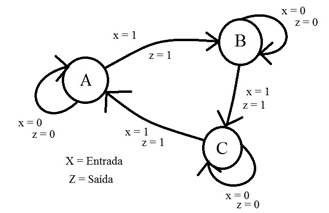
\includegraphics[width=.5\textwidth]{img/p4/fig2MaquinaMealy.png}
\caption{Exemplo de diagrama de estados usando uma máquina Mealy}
\label{fig:diagrama-mealy}
\end{figure}

\begin{figure}[!htbp]
\centering
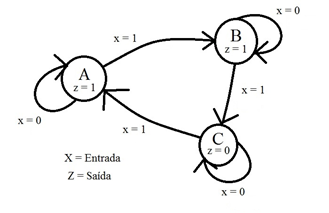
\includegraphics[width=.5\textwidth]{img/p4/fig3MaquinaMoore.png}
\caption{Exemplo de diagrama de estados usando uma máquina Moore}
\label{fig:diagrama-moore}
\end{figure}

\subsection{Flip-Flop T}

Além dos Flip-Flops até o momento estudados, temos na literatura, outro Flip-flop que é amplamente utilizado, qual seja, o Flip-flop T. Na figura~\ref{fig:fft} podemos analisar o bloco lógico e a tabela verdade para este Flip-Flop. Quando a entrada T estiver em estado alto, o flip-flop T, onde T significa \textit{toggle}, comutará quando o \textit{clock} for aplicado. Se a entrada T for baixa, o flip-flop mantém o valor do seu estado. Vale lembrar, que o Flip-flop T pode ser obtido utilizando um Flip-flop J-K, basta conectar as entradas J e K em nível lógico alto de maneira intermitente.  

\begin{figure}[!htbp]
\centering
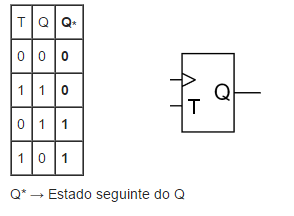
\includegraphics[width=.5\textwidth]{img/p4/fig4Flip-Flopt.png}
\caption{Tabela Verdade do Flip Flop T}
\label{fig:fft}
\end{figure}
\subsection{Flip-Flop T}

\subsection{Registrador de Deslocamento}

No universo dos circuitos digitais, principalmente no que diz respeito aos Flip-Flops, encontramos diversas aplicações. Uma, das várias aplicações é na forma de registrador de deslocamento, os quais são amplamente utilizados hoje em dia no desenvolvimento de circuitos robustos. Segundo \cite{floyd2011digital} os registradores de deslocamento consistem de arranjos de Flip-Flops e são importantes em aplicações que envolvem o armazenamento e a transferência de dados em sistemas digitais. É importante esclarecer, que o funcionamente do registrador de deslocamento é diferente de um contador comum, ou seja, ele não tem uma sequência específica de estados, apesar de em alguns casos poder ser utilizado como tal. Na figura~\ref{fig:rdeslocamento} podemos ver um circuito típico para um registrador de deslocamento de quatro bits com entrada e saída serial de dados.

\begin{figure}[!htbp]
\centering
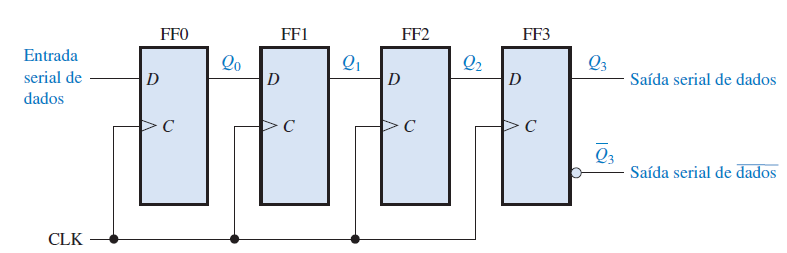
\includegraphics[width=.5\textwidth]{img/p4/Fig5RegistradorDeslocamento.png}
\caption{Representação de um registrador de deslocamento de 4 bits \cite{floyd2011digital}}
\label{fig:rdeslocamento}
\end{figure}


\subsection{Flip-Flop T}

São diversos, os tipos de registradores de deslocamento, na figura~\ref{fig:registradores} pode-se observar os diversos tipos de registradores de deslocamento existentes, sendo ilustrados de forma abstrata. Dentre eles, um dos mais importantes está o registrador com entrada serial e saída paralela, o qual será abordado com mais detalhe na próxima sub-subseção.

\begin{figure}[!htbp]
\centering
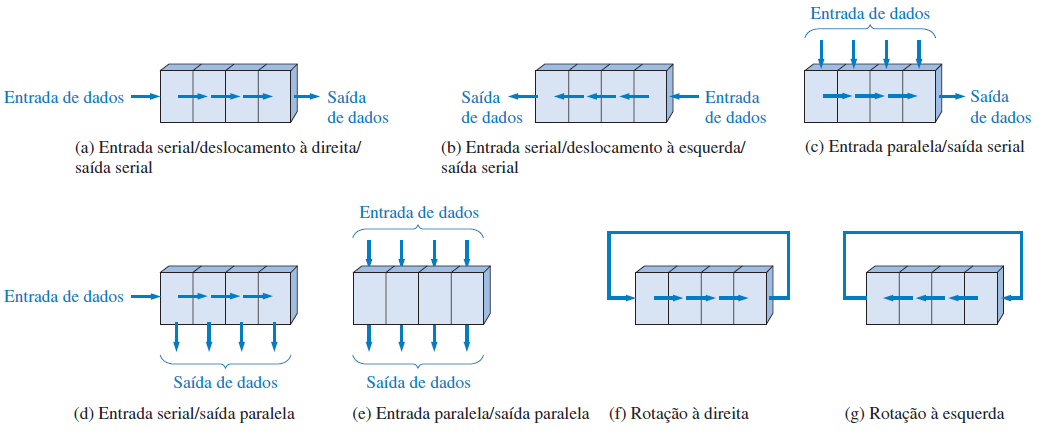
\includegraphics[width=.5\textwidth]{img/p4/Fig6tipodeRegistrador.png}
\caption{Diferentes tipos de registradores, segundo \cite{floyd2011digital}}
\label{fig:registradores}
\end{figure}

\subsubsection{Registrador de deslocamento com entrada serial e saída paralela}

Como o próprio nome já designa, neste tipo de registrador a entrada de dados se dá de forma serial, contudo, a saída não será serial e sim paralela. Desta forma, segundo \cite{floyd2011digital} uma vez armazenados os dados, cada bit aparece em sua linha de saída respectiva e todos os bits são disponibilizados simultaneamente, em vez de um bit de cada vez como no registrador com saída serial. Na figura~\ref{fig:registradorsp} podemos ver uma exemplificação para este circuito. Notem que neste tipo de registrador a saída de cada estágio está disponível.

\begin{figure}[!htbp]
\centering
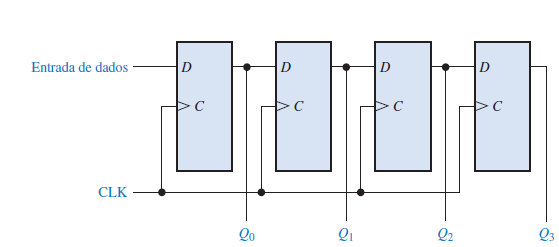
\includegraphics[width=.5\textwidth]{img/p4/Fig7RegistradorSerialParalelo.png}
\caption{Registrador Serial-Paralelo}
\label{fig:registradorsp}
\end{figure}

\subsection{Comunicação Serial}
No contexto computacional, temos duas formas de comunicação principais, são elas: comunicação serial e comunicação paralela. cada uma com suas vantagens e desvantagens. Na comunicação paralela os bits são transferidos de maneira simultânea, conferindo para este tipo de comunicação a vantagem de rapidez e simplicidade de interface, contudo essa mesma vantagem acaba gerando algumas desvantagens, pois há um maior número de conexões, o que pode gerar ruído, perda de sincronismo além de um custo maior. Já na comunicação serial os dados são transferidos  bit a bit, conferindo a vantagem de se ter menos fios, ou seja, baixo custo, além de ser capaz de transmitir dados em distâncias maiores. Contudo, nesta forma de comunicação, justamente por haver apenas um fio que transmite os dados, ela acaba sendo mais lenta, e com um grau de complexidade maior. Todavia, apesar das desvantagens da comunicação serial, a mesma se mostra mais robusta e mais viável, a ser aplicada em sistemas onde a confiabilidade dos dados são importantes. Assim, esta subseção tratará especificamente deste tipo de comunicação. 

\subsubsection{Transmissão de Dados}
Antes de falarmos acerca de como ocorrer a transmissão de dados de forma serial, é importante lembrar que existe diversas interfaces que empregam este tipo de comunicação, entre as interfaces mais antigas estão as portas $DB9$ e $DB25$, as quais podem ser encontradas nos computadores mais antigos. Na figura~\ref{fig:db9db25} temos um exemplo para estas duas portas. Cada pino nestas portas tem uma determinada função, podendo variar de acordo com o seu tipo. Na  figura~\ref{fig:pinosdb9} podemos ver a função de cada pino na porta $DB9$.


\begin{figure}[!htbp]
\centering
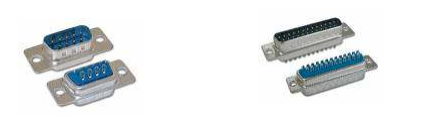
\includegraphics[width=.5\textwidth]{img/p4/fig8DB9DB25.png}
\caption{Portas DB9 e DB25, interfaces seriais encontradas em computadores antigos.}
\label{fig:db9db25}
\end{figure}

\begin{figure}[!htbp]
\centering
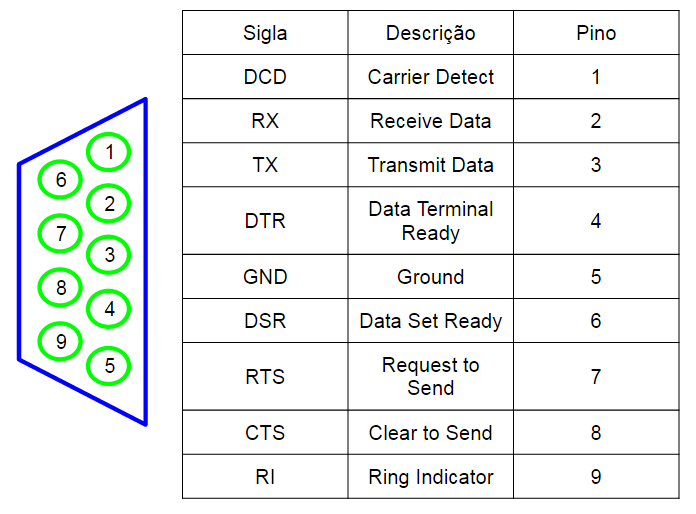
\includegraphics[width=.5\textwidth]{img/p4/Fig9serial_pinos.png}
\caption{Funcionalidades dos pinos presentes na porta DB9}
\label{fig:pinosdb9}
\end{figure}



Na maioria das aplicações, a comunicação serial acontece de forma assíncrona, onde geralmente se tem 11 bits sendo transferidos. Um desses bits é o \textit{start bit}, o qual notifica um receptor que um novo dado serial esta disponível, seguido pelos bits de dados, um bit opcional de paridade \textit{parity} e um ou mais bits de parada \textit{stop bits}\cite{porta-serial}. Percebam que o número de bits de paridade, de parada podem variar, dependendo apenas do padrão de transmissão escolhido pelo projetista. Na figura~\ref{fig:cserial} pode-se analisar esta forma de comunicação de maneira mais concreta. Vale acrescentar, que enquanto o bit de parada se manter em nível alto, os dados não estarão sendo transmitidos, e sim, apenas, quando ocorrer a mudança de estado do nível lógico alto para baixo, caracterizando assim, o bit de início, ou \textit{start bit}. 


\begin{figure}[!htbp]
\centering
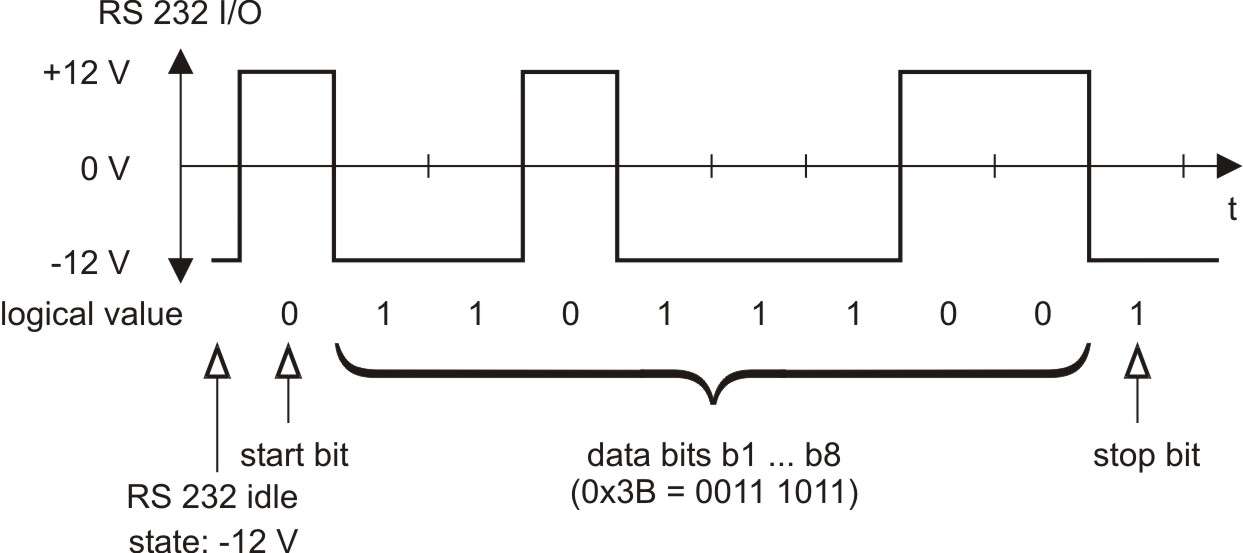
\includegraphics[width=.5\textwidth]{img/p4/Fig10rs232.jpg}
\caption{Características de uma transferência de dados serial.}
\label{fig:cserial}
\end{figure}



Cada dispositivo que emprega a comunicação serial, tem uma determinada taxa de velocidade, sendo que para se referir a velocidade de transferência devemos usar o termo bps \textit{bits-per-second}, ou seja, bits por segundo. Em alguns equipamentos, costuma-se chamar esta taxa  como \textit{baud}. Desta forma, a expressão 9600 bps é equivalente a 9600 bauds.

\subsubsection{Padrão RS-232}
Segundo (http://www.c2o.pro.br/automacao/x834.html) RS-232 é um padrão definido pela \textit{EIA-Eletronic Industries Association} para os dispositivos usados para comunicação serial. Este padrão está disponível em três versões, quais sejam, (A, B e C). Cada um especifica uma faixa de voltagens para os níveis ligado e desligado. Por exemplo, na versão RS-232 para representar  nível lógico alto utiliza-se as tensões de $-3V$ a $-12V$, enquanto para representar nível lógico baixo é utilizado tensão na faixa de $+3V$ e $+12V$. É importante notar que a representação de nível lógico alto e nível baixo nesse padrão não utiliza o modelo convencional de tensão. Vale lembrar que este padrão é utilizado marjoritariamente nas portas $DB9$ e $DB25$.  

\subsubsection{Conversor de nível MAX-232}
Os dispositivos eletrônicos utilizam níveis de tensão diferentes para identificar nível lógico baixo e nível lógico alto, dependendo apenas da tecnologia que está sendo empregada. Desta forma, quando se vai utilizar a porta serial do computador pessoal para se comunicar com algum dispositivo controlador, tem-se que analisar o padrão que o mesmo utiliza,pois a depender das especificações, será necessário fazer a conversão do nível. Por exemplo, vamos supor que queremos fazer uma comunicação entre o computador pessoal através da porta serial, com uma \textit{FPGA}. No entanto, a \textit{FPGA} utiliza a tecnologia \textit{TTL}, ou seja, 0V a 0,8V representa nível lógico baixo e $2V$ a $5V$ representa nível lógico alto. Percebe-se, assim, uma incompatibilidade entre o padrão RS-232 e o \textit{TTL}, desta forma é necessário fazer a conversão. Todavia, existe alguns dispositivos que tem a capacidade de fazer essa conversão, um deles é o MAX-232, o qual faz  a conversão entre os níveis utilizados pelo padrão RS-232 para TTL, e vice-versa. Na figura~\ref{fig:232} podemos ver uma configuração comum utilizando um conversor MAX-232. 

\begin{figure}[!htbp]
\centering
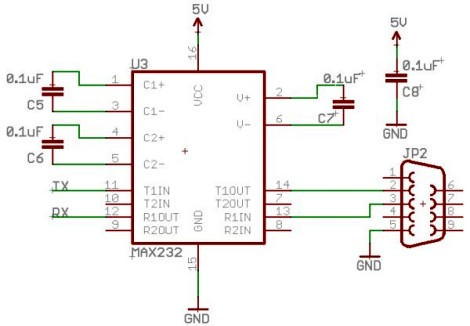
\includegraphics[width=.5\textwidth]{img/p4/Fig11-microcontroller_uart_max232_circuit.jpg}
\caption{MAX-232: Conversor de RS-232 para TTL.}
\label{fig:232}
\end{figure}

\section{Metodologia}
Utilizando-se, mais uma vez, da base teórica fornecida pela metodologia $PBL$, os alunos componentes da turma T04 iniciaram as sessões destinadas a solução do problema com a leitura do mesmo em duas etapas, uma individual e outra coletiva. Tendo como objetivo a detecção inicial de dúvidas, fatos importantes relacionados ao problema e ideias de soluções, o $brainstorm$ inicial ajudou e identificar as principais características do problema, bem assim como ter uma ideia de como iniciar o desenvolvimento do mesmo.


Os membros da sessão, solucionando as questões um dos outros quando possível durante o processo, buscaram tomar decisões de projeto para formalização das obrigações, analisando fatores positivos e negativos das soluções propostas, optando pela solução que fosse mais simples e que estivesse de acordo com o problema, de acordo com a visão dos alunos. Com esse método deu-se início a construção da solução do problema 4 do MI - Circuitos Digitais, começando pela formalização e definição de padrões de projeto e de um diagrama que as mostrasse aplicadas ao circuito.

\subsection{Decisões de Projeto}

Antes de iniciar a implementação do projeto em si, é necessário traçar o caminho a percorrer durante todo o processo de solução do problema. Essa metodologia foi adotada pelos membros da sessão após algumas decisões de projeto que não deram o resultado esperado nos problemas anteriores, causando incongruências entre os módulos projetados entre diferentes membros da turma. 

Dado o sucesso da abordagem no problema anterior, foi de comum acordo  que a turma deveria modularizar o problema e dividir tais módulos entre pequenos subgrupos, sendo que cada subgrupo deveria enviar um pequeno relatório contendo todas as informações necessárias para a elaboração do mesmo, para conscientizar os outros alunos do processo de construção, além da descrição do bloco na ferramenta EDA \textit{Quartus II 9.0}. Para garantir que, quando fossem unidos, todos os blocos funcionassem, a turma elaborou um diagrama completo do problema, estabelecendo padrões para cada segmento.

\subsection{Elaboração do Diagrama}
Iniciado na primeira sessão do problema 4 e finalizado na terceira sessão do mesmo problema, o diagrama teve como objetivo fazer com que todos os alunos tivessem consciência plena do funcionamento do circuito, da entrada à saída. Descrevendo as relações entre os blocos e a função, a quantidade de entrada e a quantidade de saídas de cada um deles e, também,  padrões de nomenclatura, o diagrama descreve o que cada subgrupo deve fazer para que, quando combinadas, as frações do problema resultem em um circuito funcional e dentro da perspectiva do problema. 

O resultado desse processo de descrição em alto nível do projeto pode ser conferido na figura~\ref{fig:diagrama}, que destaca também as tarefas de cada subgrupo. Por exemplo, o subgrupo vermelho é responsável pela elaboração dos módulos correspondentes ao \textit{comparador} e \textit{Bloco do Mux-Coordenada}.

\begin{figure}[H]
\centering
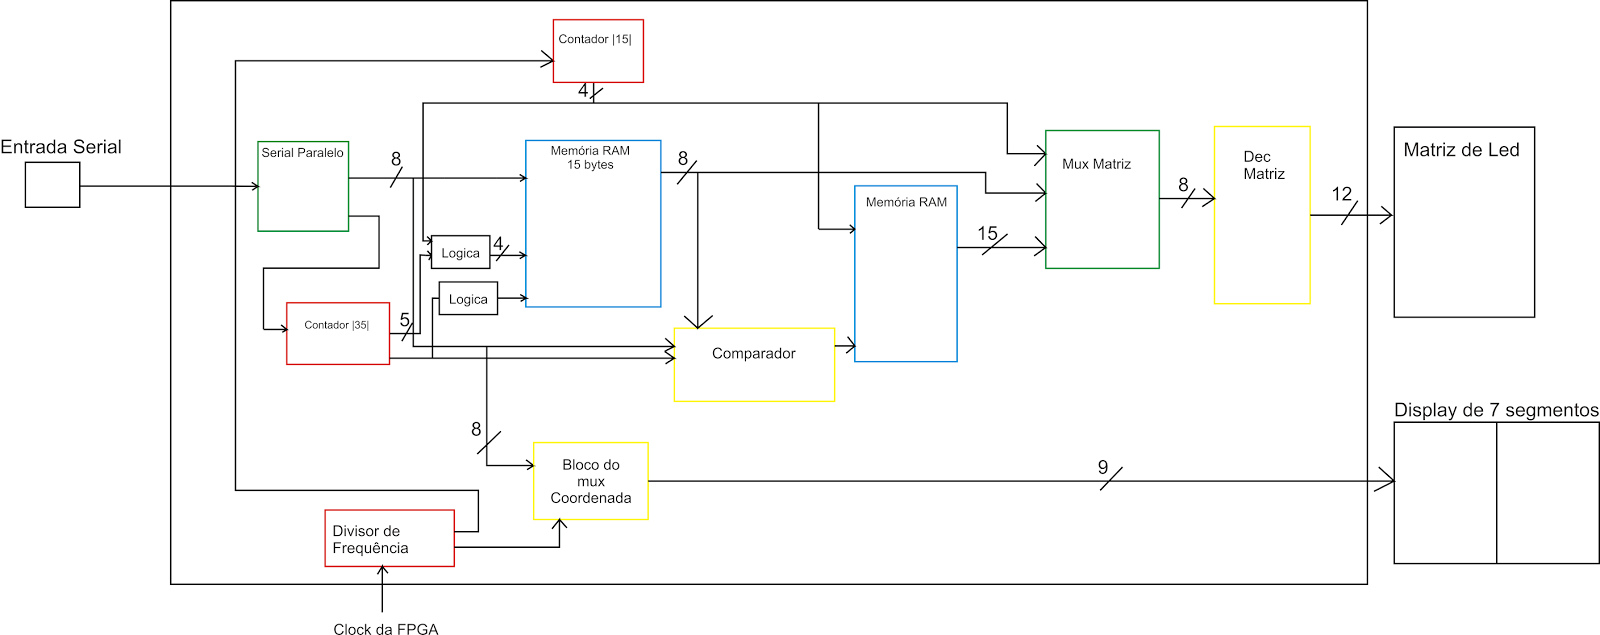
\includegraphics[width=1\textwidth]{img/p4/diagrama.png}
\caption{Diagrama de blocos do Problema 4: [COLOCAR NOME DO PROBLEMA]}
\label{fig:diagrama}
\end{figure}


\subsection{Memórias RAM}

Necessária para armazenar os dados das coordenadas inseridas na primeira etapa de jogo, armazena essas informações em um arranjo de números binários em uma célula de 1 $byte$, sendo os 4 $bits$ primeiros para informações que dizem respeito a coluna e as outras 4 $bits$, a linha.

Como explicitado nas regras determinadas pela turma(...)
[deixa q eu termino aqui]

\begin{table}[!htbp]
\centering
\begin{tabular}{||c||c||c||c||}
\hline 
\rule[-1ex]{0pt}{2.5ex} Endereço & Coordenada(CxL) & Valor Binário(C) & Valor Binário(L) \\ 
\hline 
\hline
\rule[-1ex]{0pt}{2.5ex} 0 & B,5 & 1011 & 0101 \\ 
\hline 
\rule[-1ex]{0pt}{2.5ex} 1 & B,1 & 1011 & 0001 \\ 
\hline 
\rule[-1ex]{0pt}{2.5ex} 2 & C,3 & 1100 & 0011 \\ 
\hline 
\rule[-1ex]{0pt}{2.5ex} 3 & D,5 & 1101 & 0101 \\ 
\hline 
\rule[-1ex]{0pt}{2.5ex} 4 & D,1 & 1101 & 0011 \\ 
\hline 
\rule[-1ex]{0pt}{2.5ex} 5 & E,4 & 1110 & 0100 \\ 
\hline 
\rule[-1ex]{0pt}{2.5ex} 6 & E,3 & 1110 & 0011 \\ 
\hline 
\rule[-1ex]{0pt}{2.5ex} 7 & E,2 & 1110 & 0010 \\ 
\hline 
\end{tabular} 
\caption{Informações que devem ser armazenadas e suas versões e binário}
\label{tab:ram-memory}
\end{table}



\subsubsection{Comunicação Serial}


\subsection{Transmissão de Dados}


\subsection{Comparador}


\subsection{Memória RAM}


\subsection{Multiplexador do Display Dual de Sete Segmentos} \label{sub:mux-matriz}


\subsection{Unificação dos blocos em um projeto}
Com todos os blocos prontos e devidamente testados em ambiente lógico, foram todos unidos em um único projeto e ligados como descrito no diagrama elaborado previamente. Tal tarefa foi destinada a todos os membros da equipe, como a justificativa de fortalecer o conhecimento sobre o problema e comparar e discutir os projetos em caso de eventuais discrepâncias.

\subsection{Refatoração do circuito na protoboard}


\section{Discussões e resultados}

Nesta sessão serão abordados os principais resultados obtidos, os testes realizados e, além disso, serão abordados alguns detalhes que dizem respeito ao circuito lógico.

\subsection{Testes lógicos no ambiente Quartus II}

\subsection{Funcionamento do Circuito}


\subsection{Testes práticos}
Antes de realizar os testes do circuito na Protoboard, fazia-se necessário fazer a demarcação dos pinos adicionais na ferramenta Quartus II e  gravar o circuito lógico do mesmo na FPGA disponível no laboratório. Após a demarcação dos pinos, realizada com experiência adquirida no problema 1, ligou-se o circuito e a gravação foi feita.


Dispondo-se de todas as ferramentas necessárias, o teste foi realizado introduzindo-se todas as coordenadas possíveis e tentando gravá-las na memória. Inicialmente, ao por em prática todo o planejado, foram grandes as falhas. Exibição da coordenada errada, o DSS não alternava entre seus dois estados e a matriz de LED's não acendia mesmo enviando comparações válidas. Como um resultado das práticas de projeto usadas, boa parte da equipe tinha um alto conhecimento em relação a estrutura do circuito, então, em uma revisão de todo o projeto pelo grupo, percebeu-se que tudo não passou de um descuido na hora de interligar os blocos, pois haviam diversos fios desencaixados ou encaixados no lugar errado.

Após a detecção e correção dos erros citados, o circuito funcionou como o imaginado pelo grupo, exibindo, comparando e alternando tudo que deveria na forma que deveria.


\section{Conclusão}

Observando os requisitos que foram solicitados para o desenvolvimento deste sistema digital, é notório que todas as funcionalidades foram cumpridas. Isto se torna mais concreto devido ao sucesso alcançado através dos testes práticos realizados. Em suma, todos os pré-requisitos para a elaboração do projeto das coordenadas foram obtidos com totalidade.

Tendo sido revisado várias vezes e tentando melhorar quando possível, o grupo chegou num resultado simples e funcional, e, além de tudo, totalmente compatível com o problema anterior.

Além do aspecto técnico, houve uma melhora singular no trabalho em equipe a partir do uso das práticas de projeto citadas. Problemas organizacionais, de incompatibilidade e de centralização de conhecimento, outrora frequentes, foram eliminados ou amenizados.

Apesar do circuito como um todo estar sendo melhorado, outras possíveis melhorias apontadas no problema anterior continuam não realizadas. Tal fato esclarece que tanto com iniciativas do grupo tanto como exigências do próprio problema, atualizações ainda são possíveis, como o uso de um teclado para a inserção das coordenadas e um aviso de erro mais chamativo, como um aviso sonoro(sugestão que persiste do problema anterior) e a automatização da função $comparar$ e da função $clear$, eliminando botões do sistema e o deixando sua interface com o usuário mais simples.

\section{Referências}

Nessa seção constam os trabalhos utilizados como base teórica que foram necessários para chegar a solução descrita nesse relatório.


\bibliographystyle{sbc}
\bibliography{sbc-template}

\end{document}
